\section{Evaluation}
\label{po:sec:results}

\subsection{Method}

In this section we optimize a set of numerical programs using \soap{} in a
benchmark suite with six different examples.  We use the IEEE 754 32-bit
single precision format with rounding to nearest mode as the data types of the
floating-point values used in these examples.  The benchmark consists of two
introductory numerical programs, and four real applications that are frequently
encountered in numerical analyses, and round-off errors have big impacts on the
quality of their execution.  Appendix~\ref{app:source} contains the source code
of all benchmark examples below.
\begin{itemize}

    \item \texttt{simple}: for an input $x \in [0, 20]$, we repeatedly multiply
    it with $0.9$, until the result is less than or equal to 1, the number of
    iterations is dependent on $x$ and can only be determined by analyzing the
    program.

    \item \texttt{basel}: the example in Figure~\ref{po:lst:syntax_example}.

    \item \texttt{taylor}: the Taylor expansion of $\cos(x + y)$, with single
    precision inputs $x \in [-0.1, 0.1]$ and $y \in [0, 1]$, and an integer $n
    \in [10, 20]$, which determines the bound on the iteration count.

    \item \texttt{filter}: computes the unit step response of a 3rd-order
    \gls{iir} filter, where inputs are bounded by $[0, 1]$ and all coefficients
    are bounded by $[0, 0.2]$, and it has a fixed iteration count $20$.

    \item \texttt{euler}: it uses Euler's method to solve the differential
    equation of a harmonic oscillator $\ddot{x} + \omega^2 x = 0$, with both an
    initial stationary position $x$ and $\omega^2$ bounded by $[0.0, 1.0]$, a
    step size of $0.1$, and an iteration count $n \in [0, 20]$.  It returns the
    position $x$ and velocity $\dot{x}$.

    \item \texttt{pid}: the example \gls{pid} controller that was used as a
    case study in~\cite{damouche14} as their motivation of automated accuracy
    optimization of numerical programs, we make it more challenging by changing
    constant coefficients to be bounds to model not only one, but a large
    selection of \gls{pid} controllers, with $\mathrm{kp} \in [9.0, 10.0]$,
    $\mathrm{ki} \in [0.5, 0.7]$ and $\mathrm{kd} \in [0, 3]$, and an iteration
    count $n \in [0, 20]$.

\end{itemize}

Our configuration for the efficient discovery of equivalent expressions uses a
depth limit $k = 2$, and a $D = 3$ as the maximum number of times of partial
loop unrolling.  For each program we optimize it with \soap~to discover a wide
range of implementations, and select the most accurate and least resource
demanding equivalent implementations for further analysis.  The selected
implementations are then simulated $1000$ times, with a sample of $1000$ unique
random inputs for each benchmark example, then we compare the maximum round-off
errors encountered.  Our code generator produces C source codes from the
optimized \glspl{mir}, which are then synthesized with LegUp~\cite{legup}, with
floating-point operator sharing turned off to achieve maximum frequency, then
compiled and verified with Quartus~\cite{quartus}, targeting an Altera Stratix
IV device (\textrm{EP4SGX530})~\cite{stratix4} for the actual resource usage
statistics and the frequency achieved.

\subsection{Results}

Table~\ref{po:fig:results} shows the results of optimizing the above benchmark
examples.  Here we explain the meaning of each row and column.

The rows labeled ``\texttt{FR}'' and ``\texttt{MA}'' respectively show
the statistics for the most resource efficient, and the most accurate
implementations.

The column ``Time (s)'' shows the time required for the optimization.  The
optimization runtime is longer than a typical compiler optimizer, because
during equivalent structure discovery, a significant amount of equivalent
structures are examined.

The column ``PF'' shows for each benchmark example the total number of
trade-off options in the Pareto frontier.  Larger number indicates more choices
to trade-off accuracy and area.

The values shown in the ``Error Bound'' column are the maximum absolute
errors found by \soap, while ``Simulation'' shows the actual absolute value
bound on round-off errors found during simulation, and the percentage shows
the actual accuracy improvement found in simulation of ``\texttt{MA}'' over
``\texttt{FR}''.  For each of these benchmark problems, the optimization for
accuracy of them correlates to the reduction of simulated round-off errors in
actual executions.  They all show improvements in accuracy over the original
by up to $65\%$ in actual execution.  The analyzed round-off errors are
larger than the simulated bounds, because our efficient accuracy analysis
over-approximates the worst-case round-off errors.

The ``Resources'' columns show our estimation of the number of \glspl{lut}
and \glspl{dsp} required for each of these programs, and the numbers in
brackets are the corresponding statistics obtained from Quartus synthesis.

\begin{table}[ht]
    \centering
    \caption{
        Table of optimization results.
    }\label{po:fig:results}
    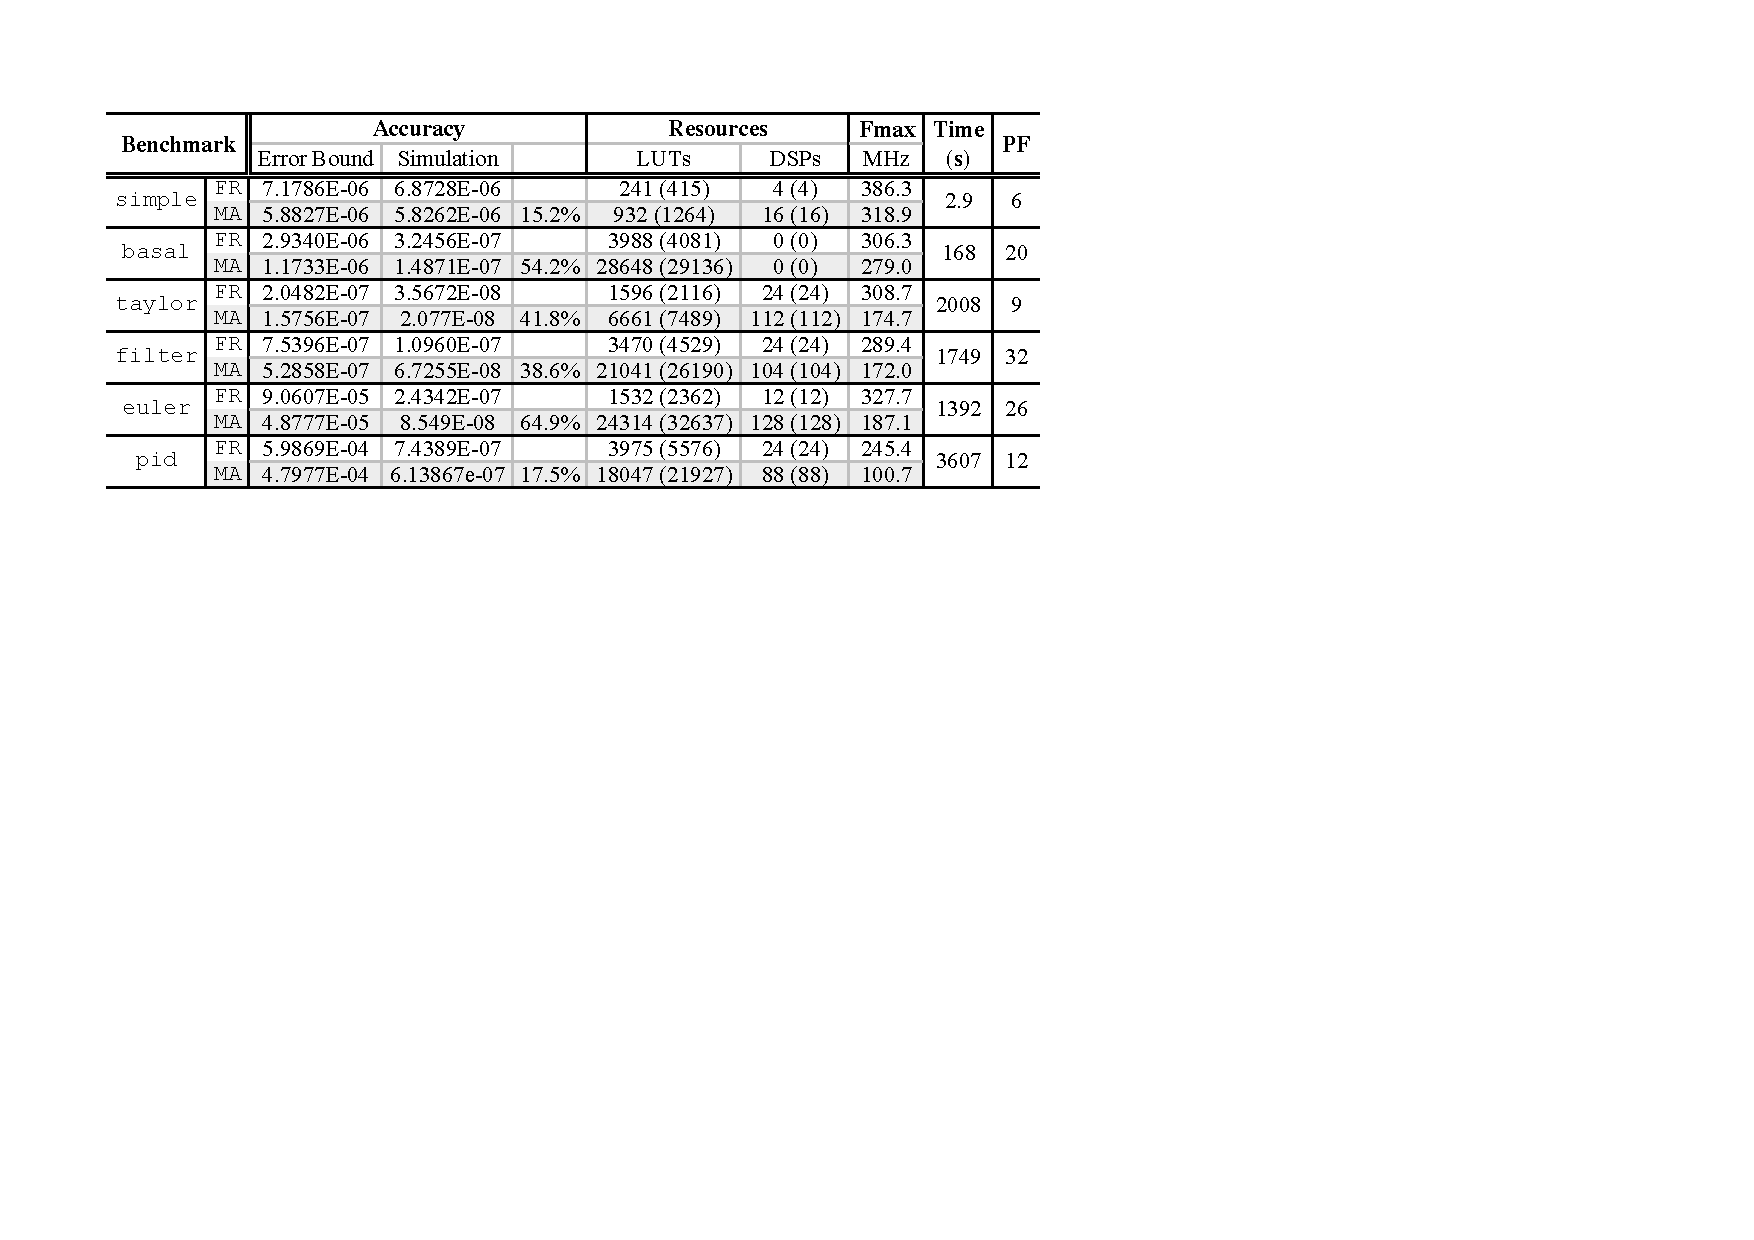
\includegraphics[width=\linewidth]{results}
\end{table}

Because our benchmark examples are designed to be resource efficient, there
is no room for resource usage optimization of the original program.  However
we are able to consistently reduce the resource usage of a plain partial
loop unrolling by more than 25\%, because our optimization can discover
subexpression sharing opportunities, propagate constants values, and also
aggressively reduce the size of expressions by powerful reduction rules such as
$e - e = 0$ and $0 \times e = 0$.

Besides the choices of implementations that are either most accurate or most
resource efficient, each optimization also offers a wide selection of optimized
programs on the Pareto frontier.  For instance, Figure~\ref{po:fig:euler}
shows the Pareto frontier of \texttt{euler}, which has 26 different trade-off
options.  Furthermore, in the optimization of \texttt{euler}, our optimization
not only identifies that it is resource efficient when the two return variables
are computed by the same loop, but also by individually optimizing the
accuracy of the two variables, we produce a program with two loops, each with
a different goal, that is to compute their respective return variables as
accurately as possible, this generated a program that consists of two loops
that have completely different structures.  With this, we further widen the
trade-off curve with the most accurate option improving the accuracy by 65\%.
In Figure~\ref{po:fig:filter}, because the loop kernel of \texttt{filter}
has the expression:
\begin{equation}
    \sum_{i=0}^2{\left( a_i y_{i+1} + b_i x_i \right)},
\end{equation}
which has a large number of equivalent expressions, without increasing the
resource usage, our optimization improves its accuracy by 14.5\%.

Moreover, points within the shaded region are Pareto-optimal as they optimize
\gls{dsp} count, since our Pareto frontier has three dimensions, which are
respectively accuracy, \gls{lut} utilization and the number of \glspl{dsp}.

\begin{figure}[ht]
    \centering
    \subfloat[\texttt{euler}]{%
        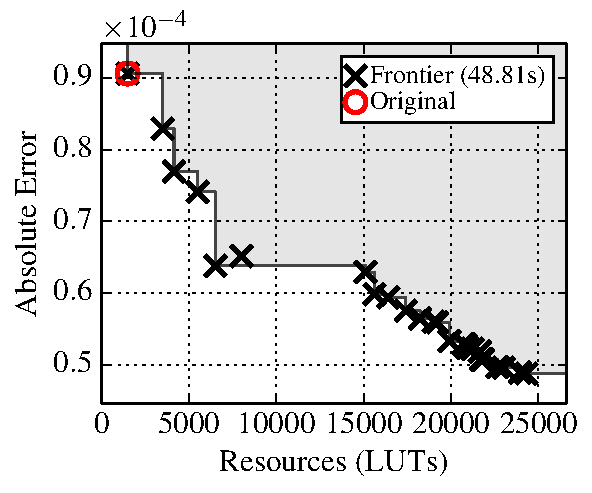
\includegraphics[width=0.6\linewidth]{euler}
        {}\label{po:fig:euler}
    } \\
    \subfloat[\texttt{filter}]{%
        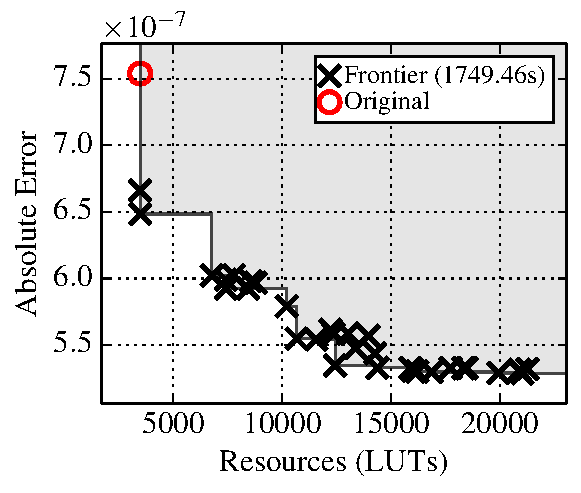
\includegraphics[width=0.6\linewidth]{filter}
        {}\label{po:fig:filter}
    }
    \caption{The Pareto frontier.}
\end{figure}

\subsection{Quality of Resource Estimation}

The Pareto frontier is sensitive to how the quality metrics of each point
(\eg~\glspl{lut}) compare against each other (\ie~the rank), while the actual
number of the metrics is irrelevant.  The Pareto frontier therefore is
unaffected if the quality metrics are perturbed by a small error such that
the rank is unchanged.  To ensure that the resource estimation method used in
our optimization can identify accurately whether an actual implementations
is on the Pareto frontier, we gathered 150 implementations discovered
across the benchmark examples, and for each one we rank its number of
estimated \glspl{lut} among them, and do the same for actual \glspl{lut}.
Figure~\ref{po:fig:rank} plots for each implementation, the rank of estimated
\glspl{lut} against the rank of actual \glspl{lut}, which shows ranking of
the resource estimation we produce is very close to the Quartus synthesized
circuits.
\begin{figure}[ht]
    \centering
    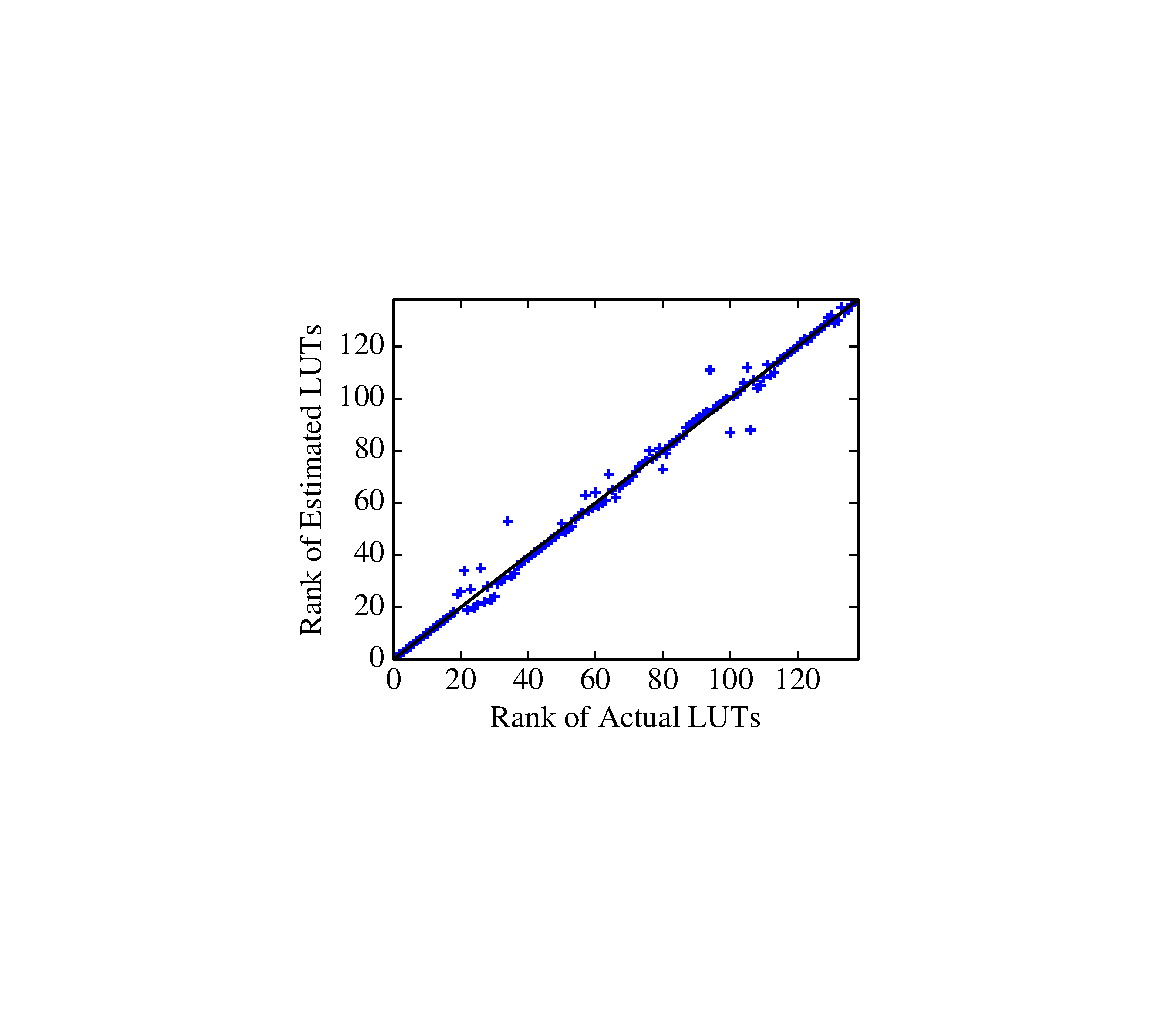
\includegraphics[scale=0.7]{rank}
    \caption{%
        The quality of resource estimation.
    }\label{po:fig:rank}
\end{figure}
